\chapter*[Metodologia]{Metodologia}
\addcontentsline{toc}{chapter}{Metodologia}

O presente capítulo possui como objetivo apresentar o detalhamento metodológico que orienta a execução deste trabalho, ao longo das suas etapas. Primeiramente, a pesquisa é classificada em relação à sua abordagem, natureza, objetivos e procedimentos. Logo após, apresenta-se  o fluxo de atividades realizadas para a realização deste projeto. O esquema mostrará a visão geral dos processos que são necessários para a criação e desenvolvimento do trabalho. Por fim, é apresentado as considerações finais do capítulo.

\section{Fluxo das Atividades}

O projeto foi desenvolvido em etapas, que serão apresentadas nessa seção ainda. Procurando apresentar o processo no geral, para os escopos definidos para o TCC-01 e o TCC-02, usou-se um modelo com a notação BPMN \cite{bpmn}, Figura \ref{fig09}, com foco no fluxo de tarefas.

    \begin{figure}[!h]
    	\centering
    	\caption{Modelo BPMN do fluxo de atividades}
    	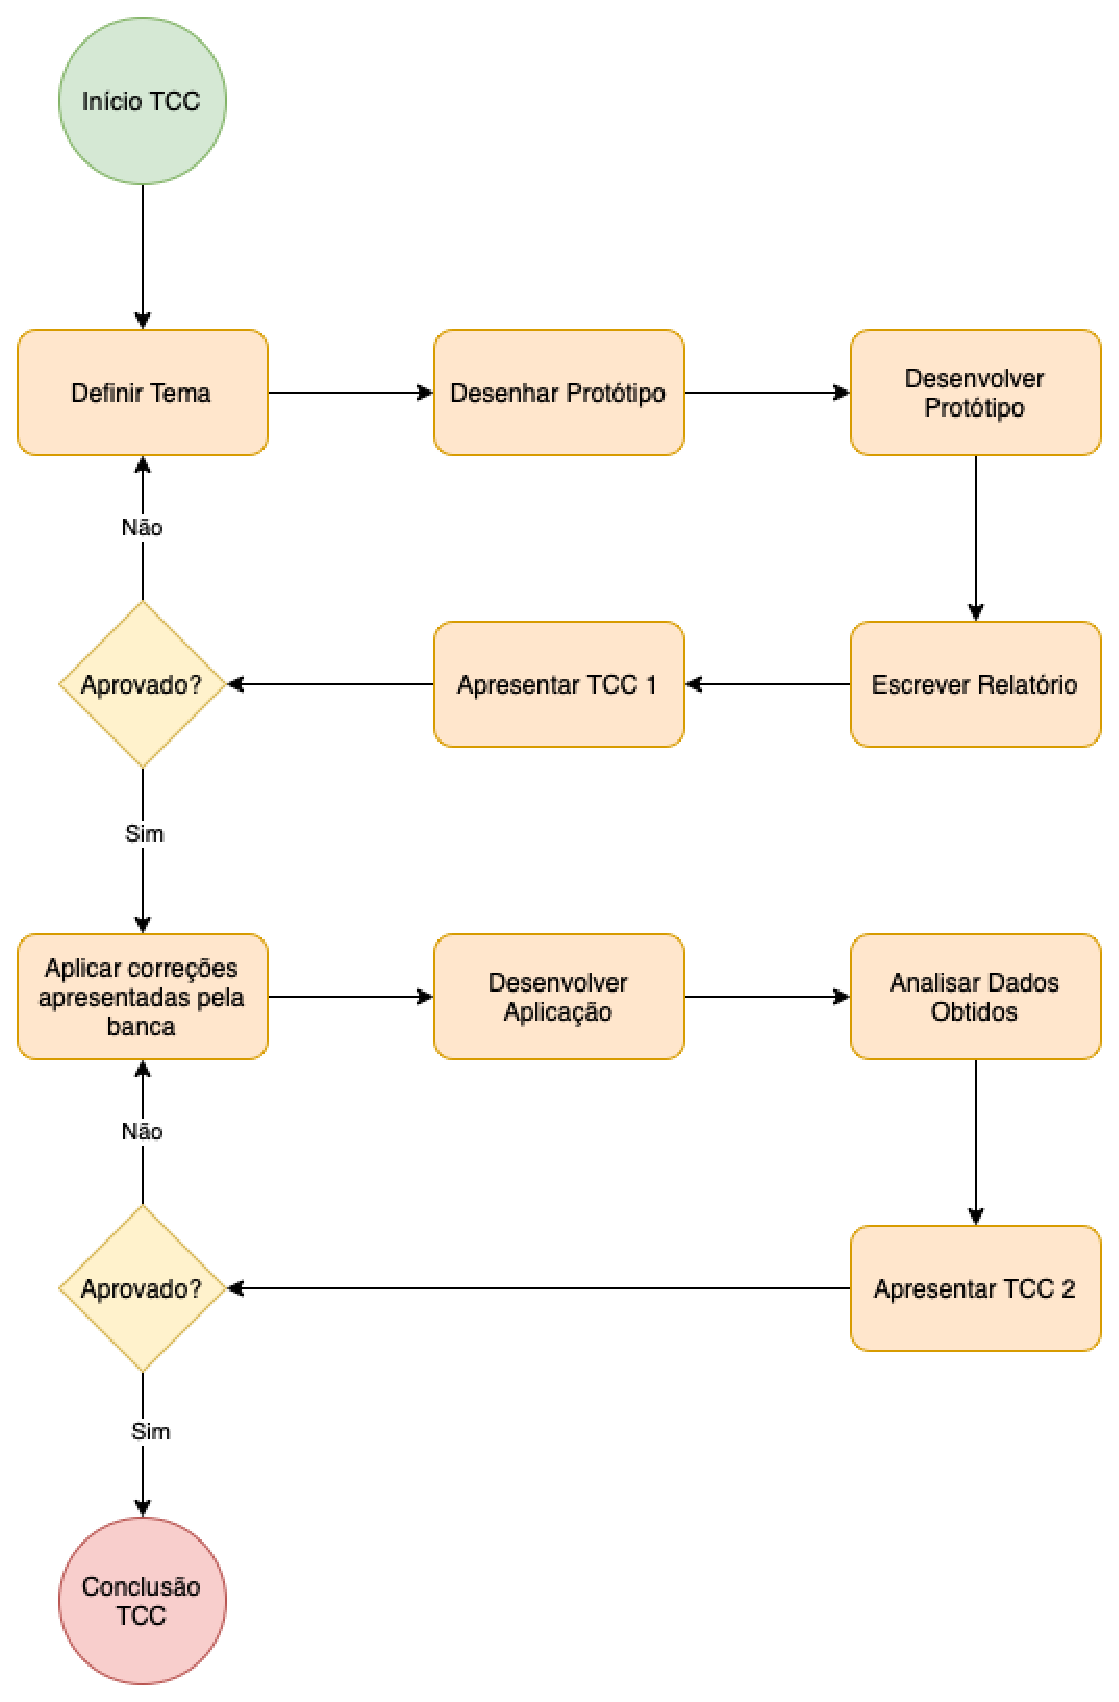
\includegraphics[keepaspectratio=true,scale=0.4]{figuras/metodologia.eps}
    	\label{fig09}
    \end{figure}
    
\begin{itemize}
		\item \textbf{Definir tema}: atividade realizada e acompanhada pelo orientador. Essa etapa tem a finalidade de estabelecer qual a hipótese a ser explorada pelos autores.
		\item \textbf{Desenhar Protótipo}: atividade em que a arquitetura da solução é pensada e desenhada.
		\item \textbf{Desenvolver Protótipo}: atividade em que um protótipo da solução é desenvolvido, e a viabilidade do tema proposto é comprovada.
		\item \textbf{Escrever Relatório}: atividade onde o referencial teórico é coletado, as ideias da proposta são apresentadas, o protótipo é descrito, e os próximos passos são descritos.
		\item \textbf{Apresentar TCC 1}: atividade não realizada. Consiste na apresentação para avaliação da banca;
		\item \textbf{Aplicar correções apresentadas pela banca}: atividade não concluída. Sobre as adaptações sugeridas do trabalho de acordo com a análise feita pela banca avaliadora;
		\item \textbf{Desenvolver aplicação}: atividade iniciada. Envolve a implementação da aplicação proposta de acordo com o processo de desenvolvimento definido.
		\item \textbf{Analisar dados obtidos}: atividade não feita. Busca estudar os resultados da aplicação, analisando se a mesma cumpriu os objetivos do trabalho.
		\item \textbf{Apresentar TCC 2}: atividade não feita. A respeito da apresentação final do trabalho junto à banca.
\end{itemize}

\section{Metodologia de Desenvolvimento}

O processo de desenvolvimento do \textit{software} proposto será realizado dentro das fases apresentadas no modelo BPMN, ilustrado na Figura \ref{fig10}. Cada etapa de desenvolvimento é executado segundo o fluxo de atividades abaixo:

\begin{itemize}
		\item \textbf{\textit{Backlog} do produto}: é o artefato que procura agrupar todos os requisitos da aplicação entre outras tarefas necessárias para o desenvolvimento da aplicação;
		\item \textbf{Fazer}: atividades priorizadas e com o compromisso de ser desenvolvido. Pode-se alterar de acordo com a necessidade e andamento do projeto;
		\item \textbf{Fazendo}: atividades em desenvolvimento;
		\item \textbf{Revisão}: atividades finalizadas e que devem ser revisadas pelo orientador ou por outro desenvolvedor para melhorias, e
		\item \textbf{Feito}: atividades concluídas e que podem ser adicionadas à versão em produção do \textit{software}.
\end{itemize}

    \begin{figure}[!h]
    	\centering
    	\caption{Modelo BPMN do fluxo de desenvolvimento}
    	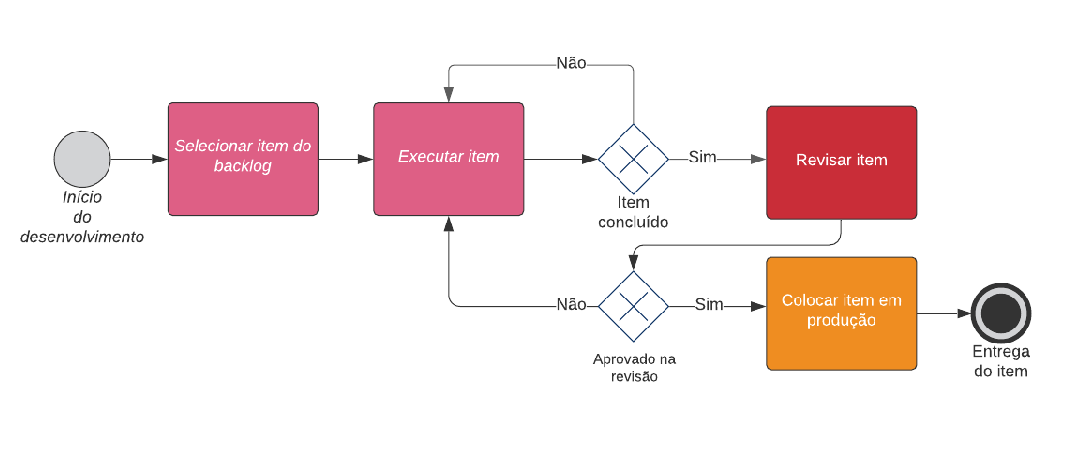
\includegraphics[keepaspectratio=true,scale=0.6]{figuras/fluxo_dev.eps}
    	\label{fig10}
    \end{figure}
    
\section{Metodologia de Análise de Resultados}

A pesquisa-ação assume "uma modalidade de pesquisa que não se ajusta ao modelo clássico de pesquisa científica, cujo propósito é o de proporcionar a aquisição de conhecimentos claros, precisos e objetivos" \cite{MetodoPesquisa}. Por isso, segue o fluxo que será usado para orientar a análise de resultados do presente projeto, ilustrado na Figura \ref{fig11}:

\begin{itemize}
		\item \textbf{Coleta de dados}: absorver e abstrair dados através de cenários de uso planejados;
		\item \textbf{Análise e interpretação dos dados}: observar os dados coletados e interpretar os dados obtidos de forma empírica;
		\item \textbf{Plano de ação}: organização de uma ação para o problema alvo da analisado, e
		\item \textbf{Divulgação dos resultados}: documentar os resultados obtidos.
\end{itemize}

    \begin{figure}[!h]
    	\centering
    	\caption{Ciclo de pesquisa-ação}
    	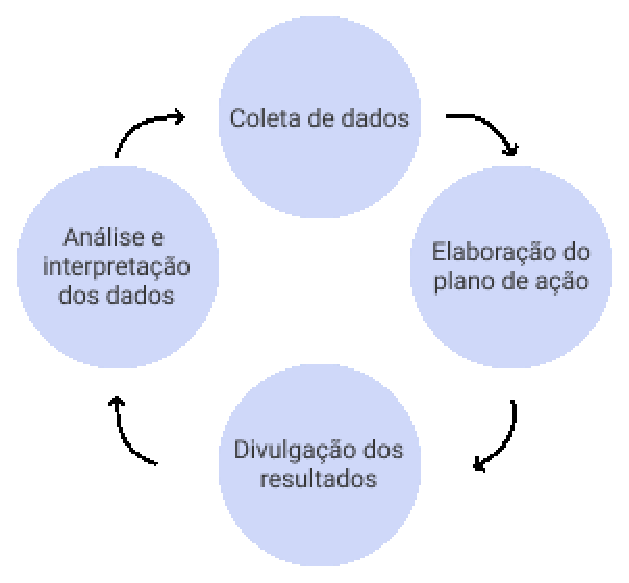
\includegraphics[keepaspectratio=true,scale=0.6]{figuras/ciclo_gil.eps}
    	\label{fig11}
    \end{figure}
    
\section{Cronograma}

A Tabela \ref{tab:cronograma_tcc} apresenta o cronograma de atividades executadas no TCC 1. Já a Tabela \ref{tab:cronograma_tcc2} acorda o cronograma preliminar de atividades previstas para serem realizadas no TCC 2.

\begin{table}[!h]
    \centering
    \caption{Cronograma do Trabalho de Conclusão de Curso 1.}
    \label{tab:cronograma_tcc}
    \begin{tabular} {c|c|c|c|c|c}
    \hline
        \textbf{Atividade} & \textbf{Jul/2021} & \textbf{Ago/2021} & \textbf{Set/2021} & \textbf{Out/2021} & \textbf{Nov/2021} \\
        \hline
        Definir tema & X &  &  &  &  \\
        \hline
        Desenhar protótipo  &  X & &  &  &  \\
        \hline
        Desenvolver protótipo  &  & & X  &  &  \\
        \hline
        Escrever Relatório  &  &  &  &  X &  \\
        \hline
        Apresentar à banca   &  &  &  &  & X \\
        \hline
    \end{tabular}
    \label{tab:cronograma_tcc}
\end{table}

\begin{table}[!h]
    \centering
    \caption{Cronograma do Trabalho de Conclusão de Curso 2.}
    \label{tab:cronograma_tcc2}
    \begin{tabular} {p{4cm}|c|c|c|c|c}
    \hline
        \textbf{Atividade} & \textbf{Jan/2022} & \textbf{Fev/2022} & \textbf{Mar/2022} & \textbf{Abr/2022} & \textbf{Mai/2022} \\
        \hline
        Aplicar correções & X &  &  &  &  \\
        \hline
        Desenvolver ferramenta  & X & X & X &  &  \\
        \hline
        Coletar e analisar resultados  &  &  &  & X &  \\
        \hline
        Apresentar à banca  &  &  &  &  & X \\
        \hline
    \end{tabular}
    \label{tab:cronograma_tcc2}
\end{table}

\section{Considerações Finais do Capítulo}

O presente capítulo apresentou todas as tomadas de decisão da metodologia do trabalho. Sendo assim, a metodologia de pesquisa deste trabalho pode ser  classificada como sendo uma abordagem qualitativa, com natureza aplicada, tendo o seu objetivo de se tornar uma pesquisa explicativa e o seu procedimento de pesquisa-ação. Finalmente, foram definidos os fluxos de desenvolvimento da aplicação e, igualmente, análise dos resultados.
